% -*- TeX-master: "oving04"; -*-
\oppgaver{6}

\begin{oppgave}
Regn ut determinanten til følgende matriser og avgjør -- basert på dette -- om kolonnene er lineært uavhengige:
\begin{punkt}
$$\begin{bmatrix}
1 & 2\\
1 & 2
\end{bmatrix}$$
\end{punkt}

\begin{punkt}
$$\begin{bmatrix}
1 & 2\\
2 & 1
\end{bmatrix}$$
\end{punkt}

\begin{punkt}
$$\begin{bmatrix}
1 & 2 & 3\\
2 & 3 & 4\\
3 & 4 & 5
\end{bmatrix}$$
\end{punkt}

\begin{punkt}
$$\begin{bmatrix}
8 & -7 & 0\\
-8 & -7 & 3\\
-4 & 5 & -8
\end{bmatrix}$$
\end{punkt}

\end{oppgave}

\begin{losning}

\begin{punkt}
0
\end{punkt}

\begin{punkt}
-3
\end{punkt}

\begin{punkt}
0
\end{punkt}

\begin{punkt}
860
\end{punkt}

\end{losning}


\begin{oppgave}
Hva er sammenhengen mellom areal/volum og determinanten? Regn ut og skisser arealet av parallellepipedet utspent av følgende vektorer i $\mathbb{R}^2$:

\begin{punkt}
$$
\begin{bmatrix}
1\\
1
\end{bmatrix} \quad \begin{bmatrix}
2\\
2
\end{bmatrix}$$
\end{punkt}


\begin{punkt}
$$
\begin{bmatrix}
1\\
2
\end{bmatrix} \quad \begin{bmatrix}
2\\
1
\end{bmatrix}$$
\end{punkt}

\end{oppgave}

\begin{losning}

\begin{punkt}
0


\begin{center}
	\begin{tikzpicture}[scale=1]
	\draw[->,above] (0,0) node{} -- (1,1) node{$\vv{1}{1}$};
	\draw[->, right] (0,0) node{} -- (2,2) node{$\vv{2}{2}$};
	%\draw[->, right] (0,0) node{} -- (2,-1) node{$\V{v}_3$};
	\draw[->] (-1,0) {} -- (3,0) {};
	\draw[->] (0,-1) {} -- (0,3) {};
	\end{tikzpicture}
\end{center}
\end{punkt}

\begin{punkt}
3

\begin{center}
	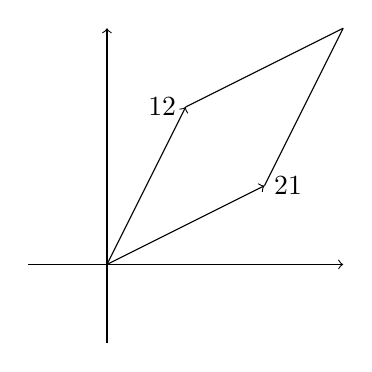
\begin{tikzpicture}[scale=1]
	\draw[->,left] (0,0) node{} -- (1,2) node{$\vv{1}{2}$};
	\draw[->, right] (0,0) node{} -- (2,1) node{$\vv{2}{1}$};
	\draw[] (1,2) node{} -- (3,3);
	\draw[] (2,1) node{} -- (3,3);
	%\draw[->, right] (0,0) node{} -- (2,-1) node{$\V{v}_3$};
	\draw[->] (-1,0) {} -- (3,0) {};
	\draw[->] (0,-1) {} -- (0,3) {};
	\end{tikzpicture}
\end{center}
\end{punkt}


\end{losning}


\begin{oppgave}
La $T$ være tetraederet i $\mathbb{R}^3$ med $(8,8,4)$, $(16,0,0)$, $(1,1,9)$ og~$(8,11,-4)$ som hjørner. Regn ut volumet av $T$.
\end{oppgave}

\begin{losning}
430

\noindent
Hint: Velg et referansepunkt og se på differansen fra de andre vektorene. Du har nå tre vektorer i $\mathbb{R}^3$ som definerer $T$. Observer at $T$ er halvparten av volumet til parallellepipedet definert av vektorene. 
\end{losning}


\begin{oppgave}
La $\V{e}_1$ og~$\V{e}_2$ være enhetsvektorene i~$\R^2$:
\[
\V{e}_1 = \vv{1}{0}
\qquad\text{og}\qquad
\V{e}_2 = \vv{0}{1}
\]
En $2 \times 2$-matrise $A$ kan beskrives ved hjelp av fire tall
$\alpha_1$, $\alpha_2$, $\theta$ og~$\varphi$, der:
\begin{align*}
\alpha_1\ &\text{er lengden av vektoren $A \V{e}_1$} \\
\alpha_2\ &\text{er lengden av vektoren $A \V{e}_2$} \\
\theta  \ &\text{er vinkelen (mot klokken) opp til vektoren $A \V{e}_1$} \\
\varphi \ &\text{er vinkelen (mot klokken) fra $A \V{e}_1$ til $A \V{e}_2$}
\end{align*}
Disse er illustrert på figuren under.
\begin{center}
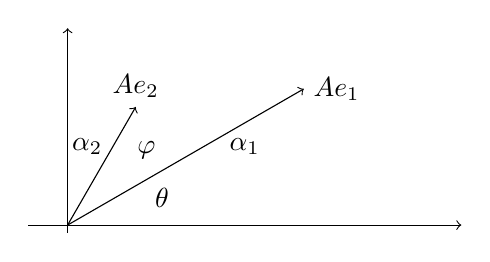
\begin{tikzpicture}[scale=.5,baseline=30pt]
\draw[->] (-1,0) -- (10,0);
\draw[->] (0,-.2) -- (0,5);
\draw[->] (0,0) -- (6,3.46);
\draw[->] (0,0) -- (1.73,3);
\node[anchor=west] at (6,3.46) {$A \V{e}_1$};
\node[anchor=south] at (1.73,3) {$A \V{e}_2$};
\centerarc[](0,0)(0:30:2);
\centerarc[](0,0)(30:60:2.3);
\node at (2.4,0.7) {$\theta$};
\node at (2,1.9) {$\varphi$};
\node at (4.5,2) {$\alpha_1$};
\node at (0.5,2) {$\alpha_2$};
\end{tikzpicture}
\end{center}
\begin{punkt}
Hvordan kan du, basert på tallene $\alpha_1$, $\alpha_2$, $\theta$
og~$\varphi$, se om determinanten til~$A$ er positiv, negativ
eller~$0$?
\end{punkt}
\begin{punkt}
Forklar hvordan determinanten til~$A$ endrer seg hvis vi endrer én av
de fire verdiene $\alpha_1$, $\alpha_2$, $\theta$ og~$\varphi$, mens
vi lar de tre andre forbli som de er.
\end{punkt}
\begin{punkt}
Finn $\det A$ uttrykt ved $\alpha_1$, $\alpha_2$, $\theta$
og~$\varphi$.
\end{punkt}
\end{oppgave}

\begin{losning}
Vi kan anta at vinklene $\theta$ og~$\varphi$ ligger i intervallet
$[-\pi,\pi)$.
\begin{punkt}
Det er kun vinkelen $\varphi$ som har noe å si for om determinanten er
positiv, negativ eller~$0$.  Determinanten er~$0$ hvis $\varphi$
er~$0$ eller~$-\pi$, og ellers har determinanten samme fortegn
som~$\varphi$.
\end{punkt}
\begin{punkt}
Hvis vi øker $\alpha_1$ eller $\alpha_2$, så øker determinanten; hvis
vi minsker en av disse, så minker determinanten.

Hvis vi varierer $\varphi$ innenfor intervallet $[-\pi/2, \pi/2]$, så
øker determinanten når $\varphi$ øker.  I intervallene $[-\pi,-\pi/2]$
og $[\pi/2,\pi)$ er det omvendt.

Å variere $\theta$ har ingen effekt på determinanten.
\end{punkt}
\begin{punkt}
$\det A = \alpha_1 \alpha_2 \sin \varphi$
\end{punkt}
\end{losning}



\begin{oppgave}
La $A$ være matrisen \[
\begin{bmatrix}
\;a & b & 0 & 0\;\\
\;c & 0 & 0 & 0\;\\
\;0 & 0 & 0 & x\;\\
\;0 & 0 & y & z\;
\end{bmatrix}.
\]
\begin{punkt}
Hva er determinanten til $A$ uttrykt ved $a, b, c$ og $x, y, z$?
\end{punkt}

\begin{punkt}
For hvilke verdier av  $a, b, c$ og $x, y, z$ er $A$ inverterbar?
\end{punkt}
\end{oppgave}


\begin{losning}

\begin{punkt}
$bcxy$
\end{punkt}

\begin{punkt}
Vi må ha at $b$, $c$, $x$ og~$y$ alle ikke er lik null.
\end{punkt}

\end{losning}

\begin{oppgave}

Avgjør om følgende påstander er sanne eller ikke. Gi et bevis eller moteksempel i hvert tilfelle.

\begin{punkt}
La $A$ og $B$ være $n\times n$-matriser. Hvis $AB$ er invertibel, så er både $A$ og $B$ invertible.
\end{punkt}

\begin{punkt}
Anta at $A$ er en inverterbar matrise. Da har vi at $$\text{det}(A^{-1})=\frac{1}{\text{det}(A)}.$$
\end{punkt}

\begin{punkt}
Hvis $A$ og~$B$ er $n \times n$-matriser, så er
\[
\det (A + B) = \det A + \det B.
\]
\end{punkt}

\begin{punkt}
Hvis $A$ og~$B$ er $n \times n$-matriser, så er
\[
\det (AB) = \det (BA).
\]
\end{punkt}

\end{oppgave}

\begin{losning}

\begin{punkt}
Sant.

\noindent
Hint: En matrise er inverterbar hvis og bare hvis determinanten ikke er lik null. Vi vet også at $\text{det}(AB)=\text{det}(A)\text{det}(B)$. Vi har antatt at $\text{det}(AB)\neq 0$. Kan du fullføre beviset?
\end{punkt}

\begin{punkt}
Sant.

\noindent
Hint: $AA^{-1}=I$ og $\text{det}(AB)=\text{det}(A)\text{det}(B)$.
\end{punkt}

\begin{punkt}
Usant.
\end{punkt}

\begin{punkt}
Sant.  Produktregelen for determinant gir:
\[
\det (AB)
 = (\det A)(\det B)
 = (\det B)(\det A)
 = \det (BA)
\]
\end{punkt}

\end{losning}


\begin{oppgave}
La $A$ være en $n \times n$-matrise, og la $\V{u}$ og~$\V{v}$ være
vektorer i~$\R^n$.  Anta at $\V{u} \ne \V{v}$, men at
$A \V{u} = A \V{v}$.  Hva kan du da si om determinanten til~$A$?
\end{oppgave}

\begin{losning}
TODO
\end{losning}


\begin{oppgave}
La $A$ være en $m \times n$-matrise slik at
\[
\det (A\tr \cdot A) \ne 0.
\]
Hva kan du da si om $m$ og~$n$?
\end{oppgave}

\begin{losning}
TODO
\end{losning}


\begin{oppgave}
La $A$ være følgende matrise:
\[
A =
\begin{bmatrix}
 3 & 0 & 2 & -2 & 1 & 0 & 1 & -1 \\
-1 & 1 & 5 &  1 & 4 & 1 & 1 &  2
\end{bmatrix}
\]
Finn $\det (A \cdot A\tr)$ og $\det (A\tr \cdot A)$.
\end{oppgave}

\begin{losning}
TODO
\end{losning}


